% 
% LaTeX Problem Set Template by Sachin Padmanabhan
% I created this when I was a freshman in CS 103,
% and I continue to use it to this day.
%
% Hope you enjoy!
%
% There may be problems with this template.
% If so, feel free to contact me.
%

% Updated for Summer 2019 by Amy Liu
% Updated for Summer 2020 by Ryan Smith

\documentclass{article}
\usepackage{amsmath}
\usepackage{amssymb}
\usepackage{amsthm}
\usepackage{amssymb}
\usepackage{mathdots}
\usepackage[pdftex]{graphicx}
\usepackage{fancyhdr}
\usepackage[margin=1in]{geometry}
\usepackage{multicol}
\usepackage{bm}
\usepackage{listings}
\PassOptionsToPackage{usenames,dvipsnames}{color}  %% Allow color names
\usepackage{pdfpages}
\usepackage{algpseudocode}
\usepackage{tikz}
\usepackage{enumitem}
\usepackage[T1]{fontenc}
\usepackage{inconsolata}
\usepackage{framed}
\usepackage{wasysym}
\usepackage[thinlines]{easytable}
\usepackage{minted}
\usepackage{wrapfig}
\usepackage{hyperref}


\title{CS 103: Mathematical Foundations of Computing\\Problem Set \#2}
\author{Your Name(s) Here}
\date{\today}

\lhead{Your Name(s) Here}
\chead{Problem Set \#2}
\rhead{\today}
\lfoot{}
\cfoot{CS 103: Mathematical Foundations of Computing --- Summer 2019}
\rfoot{\thepage}

\newcommand{\abs}[1]{\lvert #1 \rvert}
\newcommand{\absfit}[1]{\left\lvert #1 \right\rvert}
\newcommand{\norm}[1]{\left\lVert #1 \right\rVert}
\newcommand{\eval}[3]{\left[#1\right]_{#2}^{#3}}
\renewcommand{\(}{\left(}
\renewcommand{\)}{\right)}
\newcommand{\floor}[1]{\left\lfloor#1\right\rfloor}
\newcommand{\ceil}[1]{\left\lceil#1\right\rceil}
\newcommand{\pd}[1]{\frac{\partial}{\partial #1}}
\newcommand{\inner}[1]{\langle#1\rangle}
\newcommand{\cond}{\bigg|}
\newcommand{\rank}[1]{\mathbf{rank}(#1)}
\newcommand{\range}[1]{\mathbf{range}(#1)}
\newcommand{\nullsp}[1]{\mathbf{null}(#1)}
\newcommand{\repr}[1]{\left\langle#1\right\rangle}

\DeclareMathOperator{\Var}{Var}
\DeclareMathOperator{\tr}{tr}
\DeclareMathOperator{\Tr}{\mathbf{Tr}}
\DeclareMathOperator{\diag}{\mathbf{diag}}
\DeclareMathOperator{\dist}{\mathbf{dist}}
\DeclareMathOperator{\prob}{\mathbf{prob}}
\DeclareMathOperator{\dom}{\mathbf{dom}}
\DeclareMathOperator{\E}{\mathbf{E}}
\DeclareMathOperator{\Q}{\mathbb{Q}}
\DeclareMathOperator{\R}{\mathbb{R}}
\DeclareMathOperator{\var}{\mathbf{var}}
\DeclareMathOperator{\quartile}{\mathbf{quartile}}
\DeclareMathOperator{\conv}{\mathbf{conv}}
\DeclareMathOperator{\VC}{VC}
\DeclareMathOperator*{\argmax}{arg\,max}
\DeclareMathOperator*{\argmin}{arg\,min}
\DeclareMathOperator{\Ber}{Bernoulli}
\DeclareMathOperator{\NP}{\mathbf{NP}}
\DeclareMathOperator{\coNP}{\mathbf{coNP}}
\DeclareMathOperator{\TIME}{\mathsf{TIME}}
\DeclareMathOperator{\polytime}{\mathbf{P}}
\DeclareMathOperator{\PH}{\mathbf{PH}}
\DeclareMathOperator{\SIZE}{\mathbf{SIZE}}
\DeclareMathOperator{\ATIME}{\mathbf{ATIME}}
\DeclareMathOperator{\SPACE}{\mathbf{SPACE}}
\DeclareMathOperator{\ASPACE}{\mathbf{ASPACE}}
\DeclareMathOperator{\NSPACE}{\mathbf{NSPACE}}
\DeclareMathOperator{\Z}{\mathbb{Z}}
\DeclareMathOperator{\N}{\mathbb{N}}
\DeclareMathOperator{\EXP}{\mathbf{EXP}}
\DeclareMathOperator{\NEXP}{\mathbf{NEXP}}
\DeclareMathOperator{\NTIME}{\mathbf{NTIME}}
\DeclareMathOperator{\DTIME}{\mathbf{DTIME}}
\DeclareMathOperator{\poly}{poly}
\DeclareMathOperator{\BPP}{\mathbf{BPP}}
\DeclareMathOperator{\ZPP}{\mathbf{ZPP}}
\DeclareMathOperator{\RP}{\mathbf{RP}}
\DeclareMathOperator{\coRP}{\mathbf{coRP}}
\DeclareMathOperator{\BPL}{\mathbf{BPL}}
\DeclareMathOperator{\IP}{\mathbf{IP}}
\DeclareMathOperator{\PSPACE}{\mathbf{PSPACE}}
\DeclareMathOperator{\NPSPACE}{\mathbf{NPSPACE}}
\DeclareMathOperator{\SAT}{\mathsf{SAT}}
\DeclareMathOperator{\NL}{\mathbf{NL}}
\DeclareMathOperator{\PCP}{\mathbf{PCP}}
\DeclareMathOperator{\PP}{\mathbf{PP}}
\DeclareMathOperator{\cost}{cost}
\let\Pr\relax
\DeclareMathOperator*{\Pr}{\mathbf{Pr}}

\definecolor{shadecolor}{gray}{0.95}

\theoremstyle{plain}
\newtheorem*{lem}{Lemma}

\theoremstyle{plain}
\newtheorem*{claim}{Claim}

\theoremstyle{definition}
\newtheorem*{answer}{Answer}

\newtheorem{theorem}{Theorem}[section]
\newtheorem*{thm}{Theorem}
\newtheorem{corollary}{Corollary}[theorem]
\newtheorem{lemma}[theorem]{Lemma}

\renewcommand{\headrulewidth}{0.4pt}
\renewcommand{\footrulewidth}{0.4pt}

\setlength{\parindent}{0pt}

\pagestyle{fancy}
\RecustomVerbatimEnvironment{Verbatim}{BVerbatim}{}

\hypersetup{urlcolor=blue}

\renewcommand{\thefootnote}{\fnsymbol{footnote}}

% start MZ
\usetikzlibrary{automata,positioning}
\let\oldemptyset\emptyset
\renewcommand{\emptyset}{\text{\O}}
\renewcommand\qedsymbol{$\blacksquare$}
\newenvironment{prf}{{\bfseries Proof.}}{\qedsymbol}
\renewcommand{\emph}[1]{\textit{\textbf{#1}}}
\newcommand{\annotate}[1]{\textit{\textcolor{blue}{#1}}}
% end MZ

\begin{document}

\maketitle

\textbf{No checkpoint this week.}

\textbf{All Questions Due Thursday, July 9th at 11:59PM Pacific time.} \\

This second problem set explores mathematical logic. We've chosen the questions here to help you get a more nuanced understanding for what first-order logic statements mean (and, importantly, what they don't mean) and to give you a chance to practice your proofwriting. By the time you've completed this problem set, we hope that you have a much better grasp of mathematical logic and how it can help improve your proofwriting structure. \\

Before you start this problem set, we recommend that you do the following:
\begin{itemize}
	\item Familiarize yourself with the online Truth Table Tool and play around with it a bit to get a feel for the propositional connectives.
 	\item Read the online ``Guide to Negations'' and ``Guide to First-Order Translations.''
	\item Read Handout ``First-Order Translation Checklist,'' to get a better sense for common errors in first-order logic translations and how to avoid them. \emph{We will be running these checklists on your translations, so please be sure to double-check your work before submitting!}
\end{itemize}
Good luck, and have fun! \pagebreak

\section{Propositional Completeness}
In this problem, you’ll explore some redundancies within the language of propositional logic.\\

This problem is autograded and should be submitted as part of the coding component for this problem
set. Download the starter files for Problem Set Two from the course website, extract them somewhere
convenient, and edit $\mathsf{PropositionalCompleteness.proplogic}$ with your answers. There’s information
inside each file with information about how to structure your answer. Briefly, if the online Truth Table
Tool can understand your answer, so can our autograder. As usual, feel free to submit as many times as
you’d like; we’ll only grade your last submission.\\


In lecture, we covered the seven propositional connectives, which for convenience we've listed below:
$$
\neg \hphantom{--}
\land \hphantom{--} 
\lor \hphantom{--} 
\rightarrow \hphantom{--} 
\leftrightarrow \hphantom{--} 
\top \hphantom{--} 
\perp
$$
We settled on this set of connectives because they're convenient and expressive. However, it turns out that we could get away with fewer connectives than this.

\begin{enumerate}[label*=\roman*.,ref=\roman*]

    \item Show how to rewrite the expressions $\perp$ without using any connectives besides $\land$, $\lor$, $\neg$, and $\top$, along with the variables $p$ and $q$. 
    \item Repeat the above exercise for the expression $p \rightarrow q$.
    \item Repeat the above exercise for the expression $p \leftrightarrow q$.
    
    
    This means that those four propositional connectives are \emph{sufficient} -- the other three connectives can be rewritten purely in terms of them.
        
    \item There's even some redundancy in the four connectives you've used so far! Show how to rewrite the expression $p \lor q$ without using any connectives besides $\land$, $\neg$, and $\top$, along with the variables $p$ and $q$. This shows that those three connectives are actually all you need to cover all possible formulas.

\end{enumerate}

We can push this further. You can rewrite any propositional formula using just the $\rightarrow$ and $\perp$ connectives.

\begin{enumerate}[resume*]
    
    \item Find a formula that's equivalent to $\top$
    that uses only the $\rightarrow$ and $\perp$ connectives.
    
    
    \item Find a formula that's equivalent to $\neg p $ and uses only the variable $p$ and the $\rightarrow$ and $\perp$ connectives.
    
    
    \item Find a formula that's equivalent to $p \land q$
    that uses only the variables $p$ and $q$ and the $\rightarrow$
    and $\perp$ connectives.
    
\end{enumerate}

\annotate{As a hint, what happens if you negate an implication?} \\

To recap: given the $\rightarrow$ and $\perp$ connectives, you can express $\land$, $\neg$, and $\top$. From $\land$, $\neg$, and $\top$ you can get $\land$, $\lor$, $\neg$, and $\top$. And from those four connectives, you can get back the original seven. Overall, any propositional formula can be expressed purely in terms of $\rightarrow$ and $\perp$. Nifty!

\begin{shaded}
  Submit your edited $\mathsf{PropositionalCompleteness.proplogic}$ file
  through Gradescope under ``Problem Set 2 Code''.
\end{shaded}

\pagebreak

\section{Set Theory and Propositional Logic}

(Parts (i) -- (v) of this question are autograded; please edit the file
$\mathsf{SetTheory.proplogic}$ in the Problem Set Two starter files with your
answers. Part (vi) should be submitted as part of your written answers.)

Imagine we have two sets $A$ and $B$ and some object x. Let's introduce two
propositional variables:
\begin{itemize}
  \item $a$, which states that $x \in A$, and
  \item $b$, which states that $x \in B$.
\end{itemize}

By combining $a$ and $b$ together in different ways using propositional logic,
we can express different claims about how $x$ relates to $A$ and $B$.

\begin{enumerate}[label*=\roman*.,ref=\roman*]
    \item Write a statement in propositional logic using the variables $a$ and $b$ that says $x \in A \cap B$.
    \item Write a statement in propositional logic using the variables $a$ and $b$ that says $x \in A \cup B$.
    \item Write a statement in propositional logic using the variables $a$ and $b$ that says $x \in A - B$.
    \item Write a statement in propositional logic using the variables $a$ and $b$ that says $x \in A \Delta B$. To receive credit, your solution should use at most two connectives. 
\end{enumerate}

\annotate{We care about the total number of connectives you use, not how many different types of connectives you use. For example, the formula $p \land q \land r \land s \rightarrow t$ has four connectives.}\\

Now, suppose we have some third set $C$. Let's introduce a third propositional
variable $c$ that means $x \in C$.

\begin{enumerate}[label*=\roman*.,ref=\roman*]
  \setcounter{enumi}{4}
  \item Write a statement in propositional logic that says $x \in A \Delta B \Delta C$. To receive credit, your solution should use at most two connectives. (Note that $A \Delta B \Delta C = (A \Delta B) \Delta C = A \Delta (B \Delta C).)$
  
\end{enumerate}

\annotate{If you've solved part (iv), you should be able to get a solution that uses four connectives. By rewriting parts of the expression, you can then drop down to two.}

\begin{shaded}
  For parts (i) -- (v), submit your edited $\mathsf{SetTheory.proplogic}$ file
  through Gradescope under ``Problem Set 2 Code''.
\end{shaded}



\begin{enumerate}[label*=\roman*.,ref=\roman*]
\setcounter{enumi}{5}
  \item Using your answer to part (v) as a starting point, simplify the
    expression $(A \Delta B) \Delta B$ as much as possible. Briefly justify your
    answer. No formal proof is necessary. \textit{(Please write up your solution
    to this problem in your written assignment submission, since we want to see
    your justification in ad- dition to your answer.)}
\end{enumerate}
\begin{shaded}
  Write your answer here.
\end{shaded}

Generally speaking, if you ever find yourself in possession of a strange
set-theoretic expression involving the set combination operations $\cap$,
$\cup$, $-$, or $\Delta$, you can use the above technique to get a slightly
better handle at what you're looking in fact. In fact, many rules about how
these set-theoretic operators work follow directly from propositional logic! \\

That result in part (vi) is an interesting one. You may want to keep it in mind
for later in the quarter. \smiley{}

\pagebreak

\section{Executable Logic}
This problem, and the ones after it, concern worlds populated by cats, robots, and humans. Love is in the air, and for whatever reason it seems appropriate to pin down the group dynamics using first-order logic. Let's assume we have the predicates
\begin{itemize}
    \item \textit{Person(p)}, which states that $p$ is a person;
    \item \textit{Cat(c)}, which states that $c$ is a cat;
    \item \textit{Robot(r)}, which states that $r$ is a robot;
    \item \textit{Loves(x, y)}, which states that $x$ loves $y$.
\end{itemize}

As a note, the \textit{Person}, \textit{Cat}, and \textit{Robot} predicates are mutually exclusive. For example, you can’t have a robot cat or a cat person. (I mean, you can have a “cat person” in the sense that you can have a person who
likes cats, but not someone who is literally both a cat and a person. \smiley) Additionally, you can assume that each entity in the world is either a person, a cat, or a robot. Finally, note that love is not necessarily symmetric. It’s possible for $A$ to love $B$ but not the other way around. (Alas!)\\

Below is a list of six first-order logic statements. Your task is to implement the six C++ functions defined
in the file $\mathsf{ExecutableLogic.cpp}$, each of which determines whether one of the first-order logic formulas are true about a set of robots, cats, and people. Each robot, cat, or person is represented using a variable of type Entity, and we’ve provided the following C++ functions to you, which mirror the four predicates given above:

\begin{itemize}
    \item bool Person(Entity p);
    \item bool Cat (Entity c);
    \item bool Robot (Entity r);
    \item bool Loves (Entity x, Entity y);
\end{itemize}

Our provided starter files will run the six functions you’ll implement on some sample worlds, which you
can use to test out your implementations.

\begin{enumerate}[label*=\roman*.,ref=\roman*]
    \item Consider the following first-order logic formula:
    \[ \exists x.\ Cat(x) \]
    Write C++ code for a function
    \begin{center}
        bool isFormulaTrueFor\_partI(std::set<Entity> S)
    \end{center}
    that takes in a set $S$ and returns whether the above formula is true for the entities in that set.
    \item Repeat the above exercise with this first-order logic formula:
    \[ \forall x.\ Robot(x)\]
    \item Repeat the above exercise with this first-order logic formula:
    \[ \exists x.\ (Person(x) \land Loves(x, x)\]
    \item Repeat the above exercise with this first-order logic formula:
    \[ \forall x.\ (Cat(x) \rightarrow Loves(x, x)\]
    \item Repeat the above exercise with this first-order logic formula:
    \[ \forall x.\ (Cat(x) \rightarrow \\
        \exists y.\ (Person(y) \land \neg Loves(x, y))\\
    )
    \]
\end{enumerate}

\annotate{It's a lot easier to write code for this one if you use a helper function.}

\begin{enumerate}[label*=\roman*.,ref=\roman*]
\setcounter{enumi}{5}
\item Repeat the above exercise with this first-order logic formula:
    \[ \exists x.\ (Robot(x) \leftrightarrow \forall y.\ Loves(x, y))
    \]
\end{enumerate}

\begin{shaded}
  Submit your edited $\mathsf{ExecutableLogic.cpp}$ file
  through Gradescope under ``Problem Set 2 Code''.
\end{shaded}



\pagebreak


\section{First-Order Negations}

For each of the first-order logic formulas below,
find a first-order logic formula that is the negation of the
original statement.
Your final formula must not have any negations in it
except for direct negations of predicates.
For example,
given the formula
\begin{center}
$\begin{aligned}[t]
&\forall c.\ ((Cat(c) \rightarrow \\
&\qquad \exists p.\ (Person(p) \land Loves(p,c)\\
&),
\end{aligned}$
\end{center}

you could give the formula

\begin{center}
$\begin{aligned}[t]
&\exists c.\ (Cat(c) \ \land\\
&\qquad \forall p.\ (Person(p) \rightarrow \neg Loves(p,c)\\
&),
\end{aligned}$
\end{center}

However, you couldn't give as an answer the formula

\begin{center}
$\begin{aligned}[t]
&\exists c.\ (Cat(c) \land\\
&\qquad \neg \exists p.\ (Person(p) \land Loves(p,c)\\
&),
\end{aligned}$
\end{center}

since the inner negation could be pushed deeper into the expression.

To submit your answers, edit the file $\mathsf{FirstOrderNegations.fol}$ with your final formulas. That file contains information about how to format your answers.\\

We \emph{strongly} recommend reading
over the Guide to Negations before starting this problem.



\begin{enumerate}[label*=\roman*.,ref=\roman*]
\item
$\begin{aligned}[t]
&\forall p.\ (Person(p) \rightarrow\\
&\qquad \exists c.\ (Cat(c) \land Loves(p,c) \land\\
&\qquad \qquad \forall r.\ (Robot(r) \rightarrow \neg Loves(c, r))\\
&\qquad )\\
&)
\end{aligned}$

\item
$\begin{aligned}[t]
(\forall x.\ (Person(x) \leftrightarrow \exists r.\ (Robot(R) \land Loves(x, r)))) \rightarrow (\forall r.\ \forall c.\ (Robot(r) \land Cat(c) \rightarrow Loves(r,c)))
\end{aligned}$

\end{enumerate}

\annotate{Be careful -- make sure you understand how that formula is parenthesized before you try negating it.}

\begin{enumerate}[resume*]

\item
$\begin{aligned}[t]
&\forall c.\ (Cat(c) \rightarrow\\
&\qquad \exists r.\ (Robot(r) \land \\
&\qquad\qquad \forall x. \ (Loves(c, x) \leftrightarrow r=x)\\
&\qquad )\\
&)
\end{aligned}$

\item
$\begin{aligned}[t]
&\exists x.\ (Cat(x) \land \\
&\qquad (\forall r.\ (Loves(r, x) \rightarrow Robot(r)) \lor \forall p.\ (Loves(p, x) \rightarrow Person(p))) \\
&)
\end{aligned}$

\end{enumerate}
\begin{shaded}
  Submit your edited $\mathsf{FirstOrderNegations.fol}$ file
  through Gradescope under ``Problem Set 2 Code''.
\end{shaded}

\pagebreak


\section{This, But Not That}
Below is a series of pairs of statements about groups of cats, robots and people. For each pair, find the \textbf{\textit{absolute simplest}} world in which the first statement is true, and second statement is false. (By "absolute simplest," we mean using as few entities as possible, and having as few entities love each other as possible.)\\





To submit your answers, edit the file $\mathsf{ThisButNotThat.worlds}$ in the $\mathsf{res/}$ directory. There's information in that file about how to specify your worlds.\\\\


$    \textrm{Make this statement true} \qquad \qquad \qquad \textrm{And this statement false}\\\\$
    $\begin{aligned}[t]
    \textrm{i.} \qquad &\forall y.\ \exists x.\ Loves(x, y)
    \qquad \qquad \qquad \qquad \qquad \exists x.\ \forall y.\ Loves(x, y))\\\\
    \textrm{ii.} \qquad &\forall x.\ (Person(x) \lor Cat(x))
    \qquad \qquad \qquad (\forall x.\ Person(x)) \lor (\forall x. Cat(x))\\\\
    \textrm{iii.} \qquad &(\exists x.\ Robot(x)) \land (\exists x.\ Loves (x,x))
    \qquad \qquad \exists x.\ (Robot(x) \land Loves(x,x))\\\\
    \textrm{iv.} \qquad &(\forall x.\ Cat(x)) \rightarrow (\forall y.\ Loves(y, y))
    \qquad \qquad \forall x.\ \forall y.\ (Cat(x) \rightarrow Loves(y,y))\\\\
    \textrm{v.} \qquad &\exists x.\ (Robot(x) \rightarrow \forall y.\ Robot(y))
    \qquad  \qquad (\forall x.\ Robot(x)) \lor (\forall x.\ \neg Robot(x))\\\\
    \end{aligned}$

        

\annotate{As a hint, if you want to make a statement false, make its negation true.\\
The last one is subtle. Does the statement in the left column look fishy to you?}

\begin{shaded}
  Submit your edited $\mathsf{ThisButNotThat.worlds}$ file
  through Gradescope under ``Problem Set 2 Code''.
\end{shaded}
\pagebreak


\section{Translating into Logic}

In each of the following,  write a statement in first-order logic that expresses the indicated sentence. Your statement may use any first-order construct (equality, connectives, quantifiers, etc.), but you \textbf{\textit{must}} only use the predicates \textit{Person, Robot, Cat} and \textit{Loves}.\\

To submit your answers, edit the file $\mathsf{TranslatingIntoLogic.fol}$ with your formulas. There's information in that file about the expected format for your answers.\\

We \emph{highly} recommend reading the 
Guide to First-Order Logic Translations before starting this problem.

\begin{enumerate}[label*=\roman*.,ref=\roman*]
    \item Write a statement in first-order logic that says "robots do not love." (How sad!)

\end{enumerate}

\annotate{As a reminder, love is considered directional. Even if robots do not love, it's possible that people or cats might love robots. For example, I could love my Roomba even if it feels nothing toward me. \smiley{}}

\begin{enumerate}[resume*]

    \item Write a statement in first-order logic that says "each robot loves every cat, but no cat loves any person."
    \item Write a statement in first-order logic that says "each cat only loves itself." (Okay, I'm not that cynical about cats. But it's still a good exercise to translate this statement!)
    \item Write a statement in first-order logic that says "if you pick a person, you'll find that they love a cat if and only if they also love a robot."
    \item Write a statement in first-order logic that says "each person loves exactly two cats and nothing else." To clarify, each person is allowed to love a different pair of cats.
    \item Write a statement in first-order logic that says "no two robots love exactly the same set of cats."

\end{enumerate}

Looking for a good read on the theme of people, robots, pets and love? Check out Ted Chiang's novella \textit{The Lifecycle of Software Objects}, which explores these ideas in depth \smiley{}

\begin{shaded}
  Submit your edited $\mathsf{TranslatingIntoLogic.fol}$ file
  through Gradescope under ``Problem Set 2 Code''.
\end{shaded}

\pagebreak

\section{Tournament Champions}
Here's one more problem to help you practice your proofwriting.
It's a classic CS103 problem,
and we hope that you enjoy it! \\

\begin{wrapfigure}{l}{3.75cm}
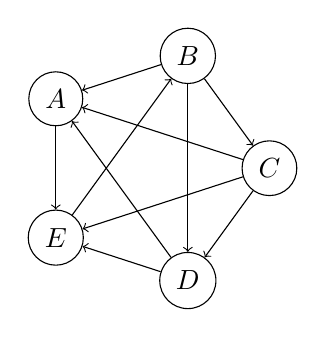
\begin{tikzpicture}[x=1.5cm, y=1.5cm]
\node[draw, circle] (C) at (1, 0) {$C$};
\node[draw, circle] (B) at
(0.30901699437494745, 0.9510565162951535) {$B$};
\node[draw, circle] (A) at
(-0.8090169943749473, 0.5877852522924732) {$A$};
\node[draw, circle] (E) at
(-0.8090169943749475, -0.587785252292473) {$E$};
\node[draw, circle] (D) at
(0.30901699437494723, -0.9510565162951536) {$D$};
\path[->] (B) edge (A);
\path[->] (C) edge (A);
\path[->] (D) edge (A);
\path[->] (A) edge (E);
\path[->] (B) edge (C);
\path[->] (B) edge (D);
\path[->] (E) edge (B);
\path[->] (C) edge (D);
\path[->] (C) edge (E);
\path[->] (D) edge (E);
\end{tikzpicture}
\end{wrapfigure}
A \emph{tournament} is a contest among $n$ players. Each player plays a game against each other player, and either wins or loses the game (let's assume that there are no draws). We can visually represent a tournament by drawing a circle for each player and drawing arrows between pairs of players to indicate who won each game. For example, in the tournament to the left, player $A$ beat player $E$, but lost to players $B$, $C$, and $D$. \\

A \emph{tournament champion} is a player in a tournament who, for each other player, either won her game against that player, or won a game against a player who in turn won his game against that player (or both). For example, in the graph on the left, players $B$, $C$, and $E$ are tournament champions. However, player $D$ is \emph{not} a tournament champion, because he neither beat player $C$, nor beat anyone who in turn beat player $C$. Although player $D$ won against player $E$, who in turn won against player $B$, who then won against player $C$, under our definition player $D$ is \emph{not} a tournament champion. \textit{(Make sure you understand why!)} \\

\begin{enumerate}[label*=\roman*.,ref=\roman*]
    \item Let $T$ be an arbitrary tournament and $p$ be any player in that tournament. Prove the following statement: if $p$ won more games than anyone else in $T$ or is tied for winning the greatest number of games, then $p$ is a tournament champion in $T$.
    
    \begin{shaded}
    Provide a proof here.
    \end{shaded}
\end{enumerate}

\annotate{This problem is a lot easier to solve if you draw the right picture. Something to think about: what happens if a player $p$ \emph{isn't} a champion in a tournament? What would that mean about player $p$? And finally, be careful not to make broad claims about tournaments or tournament structures without first proving them!} \\

\annotate{Once you've figured out the key insight and are writing up your answer, \emph{be precise with your terminology}. For example, be careful about saying something like ``player X beat player Y indirectly,'' because reasonable people can disagree about what ``indirectly'' means. For example, in the above tournament, player D beats player E, who beats player B, who beats player C, who beats player A. In one sense, that means that player D beat player A indirectly. But D isn't a tournament champion because that ``indirectly'' involves going through too many other players. If you want to talk about direct versus indirect wins, that's fine, but be sure to precisely define what you mean! Similarly, be careful about talking about different sets of players that might have some overlap. For example, ``the set of people that player C won a game against'' and ``the set of players that those people won games against'' aren't disjoint: player C beat player E, so E is in the first set, and player C also beat player A, who in turn beat player E, so player E is also in the second set.} \\

A corollary of the result you proved in part (i) is that every tournament with at least one player must have at least one tournament champion -- you can always pick someone who won the most games or is tied for winning the most games. However, note that you can be a champion without necessarily winning the most games -- for example, player $E$ in the above example tournament is a champion, though player $E$ only won a single game! \\

\begin{enumerate}[resume*]

    \item Prove that for any $n \geq 3$, there's a tournament with exactly $n$ players and exactly three champions.

    \begin{shaded}
    Provide a proof here.
    \end{shaded}
\end{enumerate}

\annotate{There's a universal and an existential component to this theorem. How do you prove existential statements?}

\section*{Optional Fun Problem: Insufficient Connectives
(Extra Credit)}

Every propositional logic formula could be written in terms of just $\rightarrow$ and $\perp$. However, you cannot express every possible propositional logic formula using just the $\leftrightarrow$ and $\perp$ connectives. Prove why not.

\begin{shaded}
Provide a proof here.
\end{shaded}

\end{document}